% !TEX root = /home/computer/ucsc/master-2/quarter-1/machine-learning/master.tex
\assignment{4}{Mon 29 Nov 2021 11:01}{Assignment 4}

\subsectionfont{\fontsize{10}{10}\selectfont}

\graphicspath{{/home/computer/ucsc/master-2/quarter-1/machine-learning/assignment_04/figures/}}

\section{Part 1}%

In the boosting algorithm I use a basic binary linear classifier on the data
$X$. Using least squares I found the slope that passes through the weighted
class exemplar $c$. 

\[
c = \frac{1}{ \sum w_i} wX
.\] 

so the least squares solution is

\[
  w_l = (X^TX)^{-1}X^{T}(y-Xc)
.\] 

and then I use this solution to find the total correctly and incorrectly
classified training points to update the weights used in the class exemplar.


The only issue I had was running this in such a way that allowed this to work
on test data that wasn't the same size as the training data. I was initially
returning the sum $ \sum \alpha_i y_{\text{pred}}$.

Here is the code

\begin{figure}[H]
  \centering
  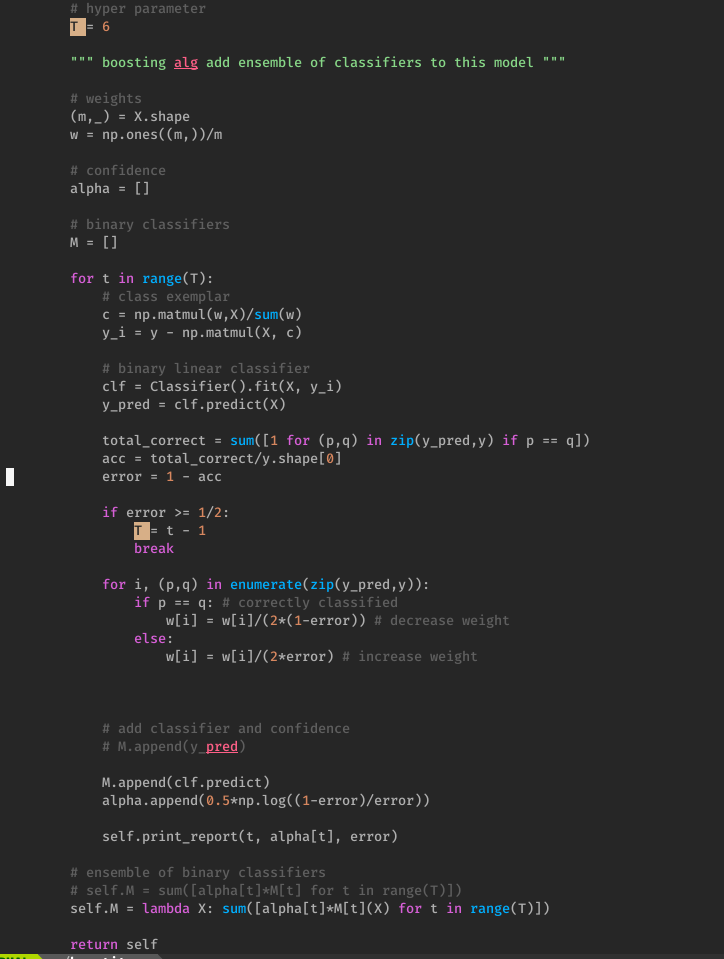
\includegraphics[width=0.8\linewidth]{boosting.png}
  \caption{Boosting}%
  \label{fig:boosting}
\end{figure}

\section{Part 2}%

Running the program for $T=5$ produces the following output

 \begin{figure}[H]
  \centering
  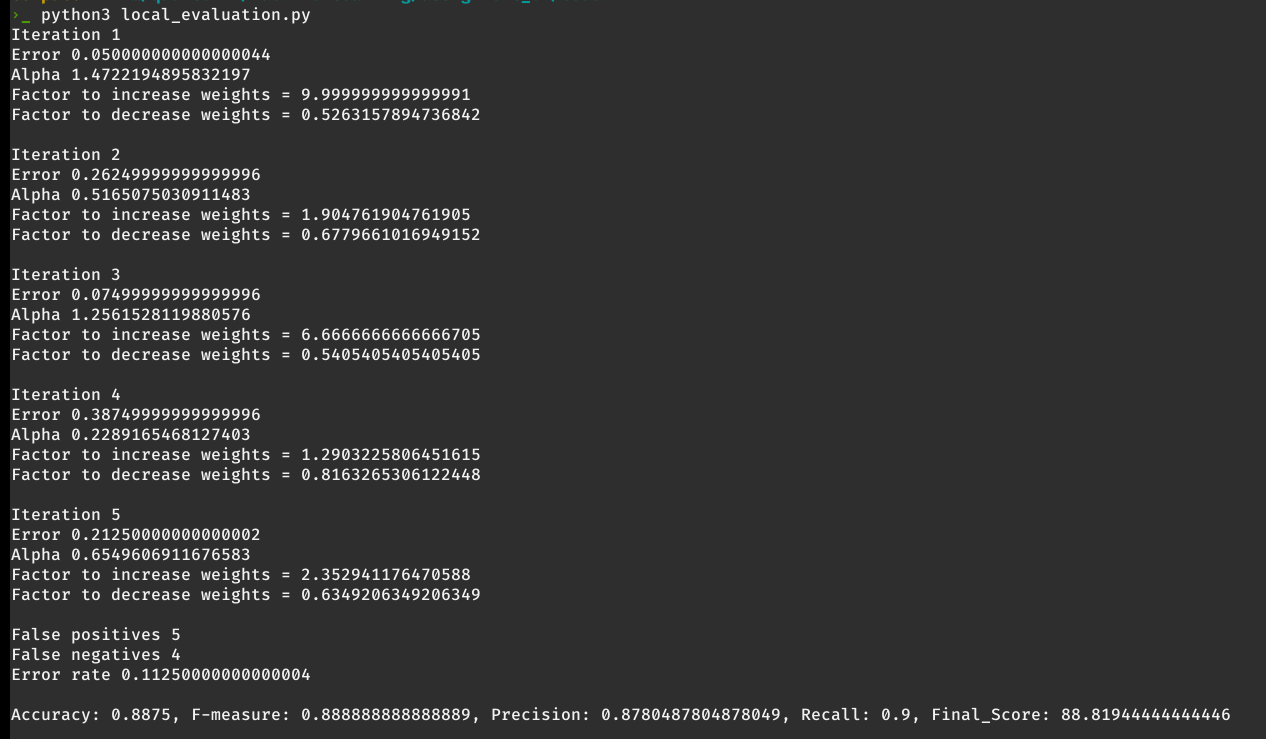
\includegraphics[width=0.8\linewidth]{part_2.png}
  \caption{Part 2}%
  \label{fig:part2}
\end{figure}

\section{Part 3}%

The result of running the program with $T=6$ is the same as the basic linear
classifier. The result for $T=5$ is shown above.

\begin{figure}[H]
  \centering
  
\includegraphics[width=0.8\linewidth]{T6.png}
  \caption{T6}%
  \label{fig:T6}
\end{figure}

I realize I should probably add additional classifiers besides the basic linear
classifier in order to give the boosting algorithm a chance to pick the
classifier that yields the smallest error.
